\documentclass[pdf]{beamer}
\usepackage[latin1]{inputenc}
\usepackage{multirow}
\usetheme{Warsaw} %Warsaw
\usecolortheme{seahorse}
\usepackage[T1]{fontenc}

\begin{document}

\title[Sequence Mapping]{Sequence Mapping/Alignment}
\subtitle{BCB 511: Applied Bioinformatics\\}
\author[Matt Settles]{Matt Settles}
\institute{University of Idaho\\ Bioinformatics and Computational Biology Program}
\date{\today}


%% Title page
\begin{frame}[plain]
  \titlepage
\end{frame}


%% Outline
\begin{frame}[plain] 
  \frametitle{Outline}
  \tableofcontents
\end{frame}

\section{Introduction}
\begin{frame}
  \frametitle{Mapping/Alignment}
Given sequence data,
\begin{description}
\item[Assembly]  seeks to put together the puzzle without knowing what the picture is 
\item[Mapping]  tries to put together the puzzle pieces directly onto an image of the picture
\end{description}
\vspace{0.1in}
In mapping the question is more, given a small chunk of sequence, where in the genome did this piece most likely come from.
\end{frame}

\begin{frame}
\begin{center}
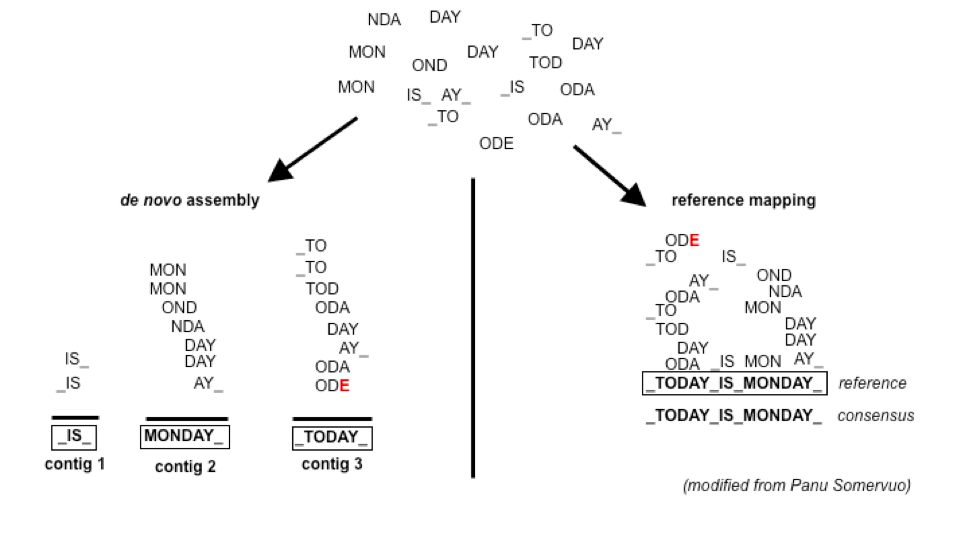
\includegraphics[scale=0.35]{Figures/Differences.png} 
\end{center}
\end{frame}

\begin{frame}[allowframebreaks]
\frametitle{The Mapping Problem}
The mapping problem:\\
\vspace{0.1in}
Given a string \textit{S} over a finite alphabet $\Sigma = \left\{A,C,T,G\right\}$, |\textit{S}| is used to
denote the length of \textit{S}, \textit{S}[\textit{i}] is the \textit{i}th character of \textit{S} and \textit{S} [\textit{i} : \textit{j}] is the substring
of \textit{S} which starts at position \textit{i} and ends at position \textit{j}. A \textit{k}-mer of \textit{S} is a
substring of \textit{S} of length \textit{k} > 0.\\
\vspace{0.1in}
The unit cost edit distance between two strings \textit{S}$_1$ and \textit{S}$_2$ is the minimum number of
substitutions, insertions and deletions required to convert
\textit{S}$_1$ to \textit{S}$_2$ refered to as EditDist(\textit{S}$_1$, \textit{S}$_2$).\\
\vspace{0.1in}
Every genomic sequence can be then be represented as a string over the alphabet $\Sigma = \left\{A,C,T,G\right\}$.
Given a genome database \textit{G} of subject sequences $\{$\textit{S}$_1$, \textit{S}$_2$, ..., \textit{S}$_n\}$,
a query sequence (read) \textit{Q} and an integer maxEditDist parameter \textit{n}, it is required to
find all substrings from \textit{G}, such that for each substring $\alpha$, EditDist($\alpha$,\textit{Q}) $<$ \textit{n}.
\\
\vspace{0.1in}
The goal then is to find the match(es) with either the "best" edit distance (smallest), or all maches with edit distance less than maxEditDist.
\vspace{0.1in}
Main issues:\\
\vspace{0.1in}
\begin{itemize}
\item Large search space
\item Regions of similarity (aka repeats)
\item Gaps (INDELS)
\item Complexity (RNA, transcripts)
\end{itemize}
\end{frame}

\section{Alignment Algorithms}
\subsection{BLAST}
\begin{frame}
  \frametitle{Basic Local Alignment Search Tool (BLAST)}
  Some say the first bioinformatics tool, developed at NIH and published in 1990.\\
  Problem:\\
  \begin{description}
  \item[-] Exact algorithms like Smith-Waterman and Needleman-Wunsch (dynamic programming) are slow, when the search space becomes large.
  \item[-] With the advent of automated DNA sequencing technology, the database of possible matches was becoming increasingly larger.
  \end{description}
  the BLAST algorithm emphasizes speed over sensitivity, and does not guarantee an optimal alignment.\\
  \alert{BLAST is a few-to-many - performs gapped alignment}
\end{frame}

\subsection{BLAT}
\begin{frame}
  \frametitle{BLAST Like Alignment Tool (BLAT)}
  Blat (Jim Kent, UCSC, 2002) was designed to solve the problem of performing comparisons between large genomes and was one of the first algorithms to efficiently search many query sequences against a large database (a genome). Blat also performs a gapped-alignment for searching RNA sequences against a genome and handling splice junctions.\\
  \begin{description}
  \item[gapped-alignment] alignment allowing for insertions and deletions greater than a few base pairs. Gapped alignment are less efficient, but more accurate.\\
  \end{description}  
  \alert{BLAT is a many-to-many algorithm - performs gapped alignments}
\end{frame}

\subsection{Improvements}
\begin{frame}
  \frametitle{Improving Algorithms}
  Many additional algorithms have been developed since BLAST and BLAT, mainly improving on either speed or accuracy, or both.
\end{frame}

\section{Illumina Data}
\begin{frame}
and then came Illumina data -\\
New Problem:\\
\begin{itemize}
\item We still have a large search space (aka genome)
\item Very small pieces, many possible close matches
\item Millions or Billions of query sequences
\end{itemize}
\end{frame}

\begin{frame}
  \frametitle{Types}
  \begin{description}
  \item[Hash based] First generation of alignment algorithms relied on hashes (Eland [Illumina], RMAP, MAQ, SHRiMP, SOAP)
  \item [Burrows-Wheeler] Second generation algorithms with a reduced memory footprint (BWA, SOAP2, Bowtie)
  \end{description}
\end{frame}

%\begin{frame}
%\begin{center}
%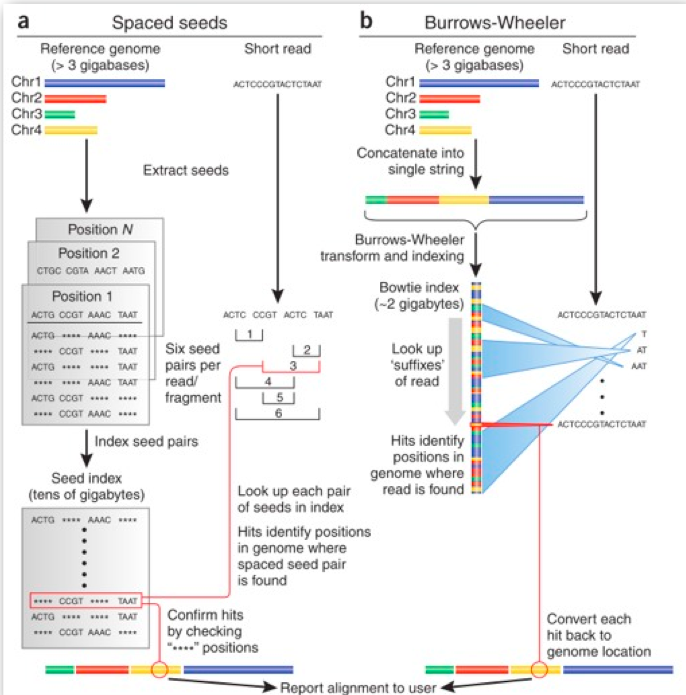
\includegraphics[scale=.32]{Figures/hashVsBW.png} 
%\end{center}
%\end{frame}

\subsection{Hash Based}
\begin{frame}
  \frametitle{hash based example: MAQ}
  \begin{itemize}
  \item  Index reference genome (or sequence reads) $=>$ creates hash index       
  \begin{itemize}
   \item Big file: $>$50GB 
   \item takes a long time (hours or overnight), but only need to do once
  \end{itemize}
  \item Divide each read into segments (seeds) and look up in table
  \begin{itemize}
  \item Search stage finds regions in the genome that can potentially be homologous to the read. 
  \item Alignment stage verifies these regions to check if they are indeed homologous. More computationally intensive
  \end{itemize}
  \end{itemize}
\end{frame}

\subsection{Burrows-Wheeler Tranform}
\begin{frame}
  \frametitle{burrows-wheeler example: Bowtie2}
   Used in data compression (e.g. bzip) $=>$ index: much smaller than hash-based index ($<$2GB)
\begin{itemize}
\item Alignment speed: 30x faster than MAQ
\end{itemize}
Steps:\\
\begin{itemize}
\item Create BWT index of genome
\item Align read 1 character at a time to BWT-transformed genome
\end{itemize}
\end{frame}

\begin{frame}
\begin{center}
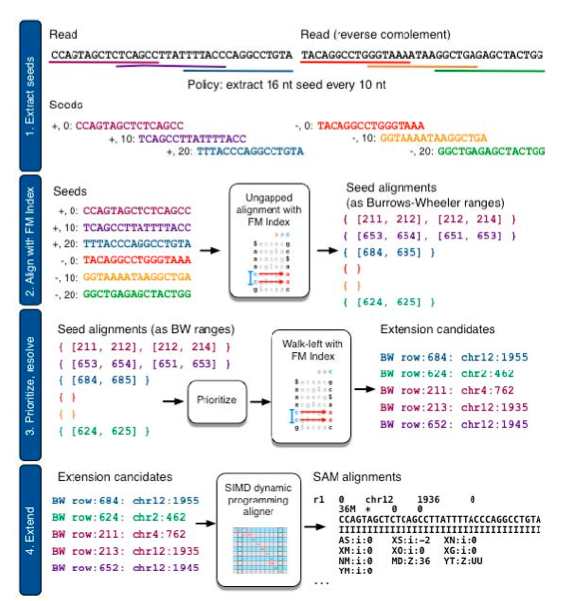
\includegraphics[scale=.35]{Figures/BWT.png} 
\end{center}
\end{frame}

\begin{frame}
\frametitle{considerations}
\begin{itemize}
\item Placing reads in regions that do not exist in the reference genome (reads extend off the end) [ mitochondrial, plasmids, etc.].
\item Sequencing errors and variations: alignment between read and true source in genome may have more differences than alignment with some other copy of repeat.
\item What if the closest fully sequenced genome is too divergent? (3\% is a common alignment capability)
\item Placing reads in repetitive regions: Some algorithms only return 1 mapping; If multiple: map quality = 0
\item Algorithms that use paired-end information $=>$ might prefer correct distance over correct alignment.
\end{itemize}
\end{frame}

\section{SAM/BAM output}
\begin{frame}
\frametitle{SAM/BAM format}
\begin{description}
\item [SAM] (Sequence Alignment/Map) format = unified format for storing read alignments to a reference genome (Consistant since Sept. 2011).\\
See http://samtools.sourceforge.net/SAM1.pdf
\item [BAM] = binary version of SAM for fast querying
\end{description}
\end{frame}

\begin{frame}
\frametitle{SAM format}
SAM files contain two regions
\begin{itemize}
\item The header section
\begin{itemize}
\item Each header line begins with character '@' followed by a two-letter record type code
\end{itemize}
\item The alignment section
\begin{itemize}
\item Each alignment line has 11 mandatory fields. These fields always appear in the same order and must be present, but their values can be '0' or '*', if the cooresponding information if unavailable, or not applicable.
\end{itemize}
\end{itemize}
\end{frame}

\begin{frame}
\frametitle{SAM Alignment lines}
SAM aligmenment lines:
\begin{center}
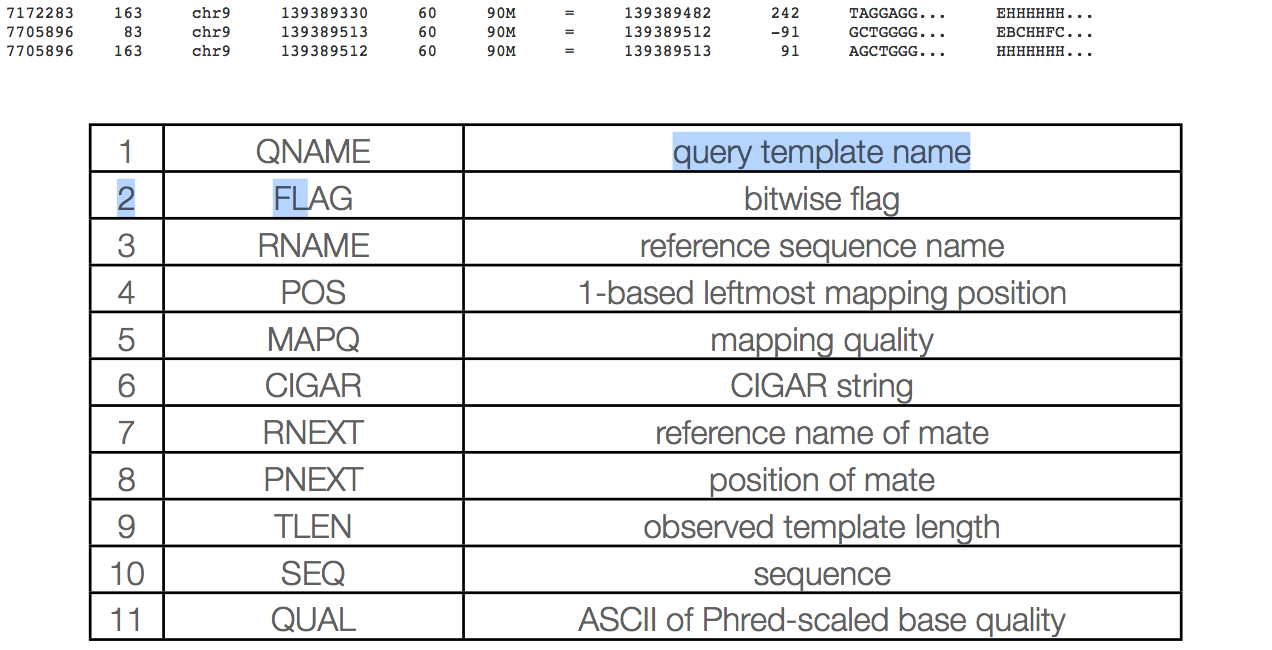
\includegraphics[scale=0.25]{Figures/sam.png} 
\end{center}
\end{frame}

\begin{frame}
\frametitle{SAM flags}
SAM flag field:
\begin{center}
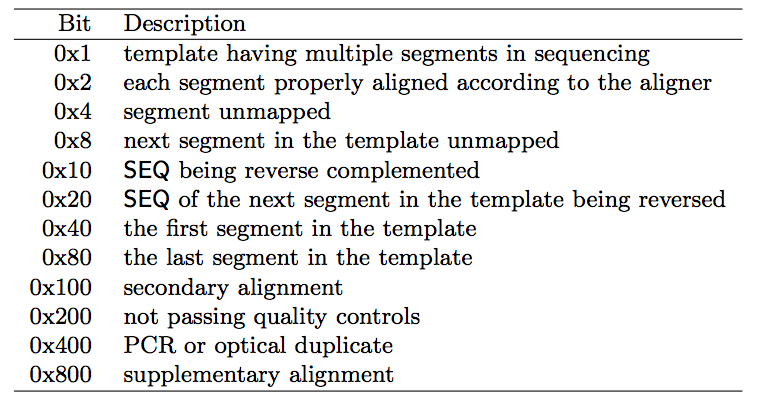
\includegraphics[scale=0.4]{Figures/Sam-flag.png} 
\end{center}
\end{frame}

\begin{frame}[allowframebreaks]
\frametitle{MAPQ explained}
MAPQ, contains the "phred-scaled posterior probability that the mapping position" is wrong.\\
\vspace{0.1in}
In a probabilistic view, each read alignment is an estimate of the true alignment and is therefore also a random variable. It can be wrong. The error probability is scaled in the Phred. For example, given 1000 read alignments with mapping quality being 30, one of them will be wrong pn average.
\vspace{0.1in}
Understanding Mapping Qualities\\
\vspace{0.1in}
The calculation of mapping qualities is simple, but this simple calculation considers all the factors below:
\begin{itemize}
\item The repeat structure of the reference. Reads falling in repetitive regions usually get very low mapping quality.
\item The base quality of the read. Low quality means the observed read sequence is possibly wrong, and wrong sequence may lead to a wrong alignment.
\item The sensitivity of the alignment algorithm. The true hit is more likely to be missed by an algorithm with low sensitivity, which also causes mapping errors.
\item Paired end or not. Reads mapped in pairs are more likely to be correct.
\end{itemize}
When you see a read alignment can get a mapping quality 30, it usually implies:\\
\begin{itemize}
\item The overall base quality of the read is good.
\item The best alignment has few mismatches.
\item The read has few or just one `good' hit on the reference, which means the current alignment is still the best even if one or two bases are actually mutations or sequencing errors.
\end{itemize}
\alert{In principle however, each mapper seems to compute the MAPQ in their own way.}
\end{frame}

\begin{frame}[allowframebreaks]
\frametitle{CIGAR explained}
Compact Idiosyncratic Gapped Alignment Report (CIGAR)
\vspace{0.1in}
SAM flag field:
\begin{center}
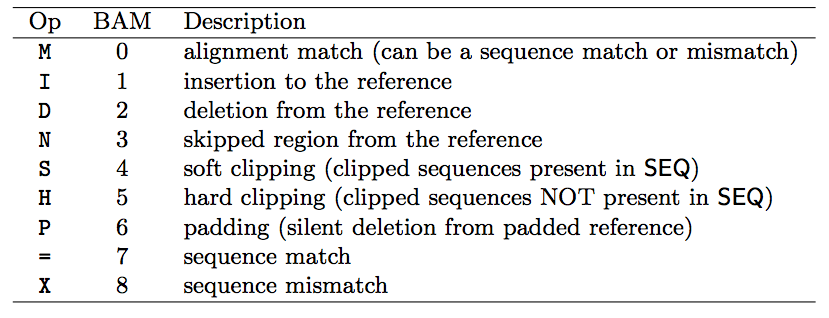
\includegraphics[scale=0.4]{Figures/Sam-Cigar.png} 
\end{center}
\end{frame}

\begin{frame}
\frametitle{CIGAR example}
RefPos: \ \ \ 1  2  3  4  5  6  7     8  9 10 11 12 13 14 15 16 17 18 19\\
Reference:  C  C  A  T  A  C  T  \   G  A  A  C  T  G  A  C  T  A  A  C\\
Read: \ \ \ \ \ \ \ \ \ \ \ \ \ \ \ \ \ \ A  C  T  A  G  A  A     T  G  G  C  T\\
\vspace{0.2in}
POS: 5\\
CIGAR: 3M1I3M1D5M\\
\end{frame}
\end{document}
